The main objectives of this water treatment device are:

\begin{itemize}

\item{} Obtaining a high degree of purification in the processed water sample, reducing its conductivity by approximately two orders of magnitude (from $1000~\mu$S$/\cm$ to $10~\mu$S$/\cm$)

\item{} Designing of a device with low maintenance (low cost  and low manpower)

\item{} Installation of a remote control devices based on probes and valves and development of a software to management it.
\end{itemize}

For this, the LARUEX laboratory in Extremadura, one of the six collaborators of the TRITIUM experiment, has designed, developed and built an ultrapure water system, a scheme of which is shown in Figure \ref{fig:WPSScheme}.

\begin{figure}[htbp]
\centering
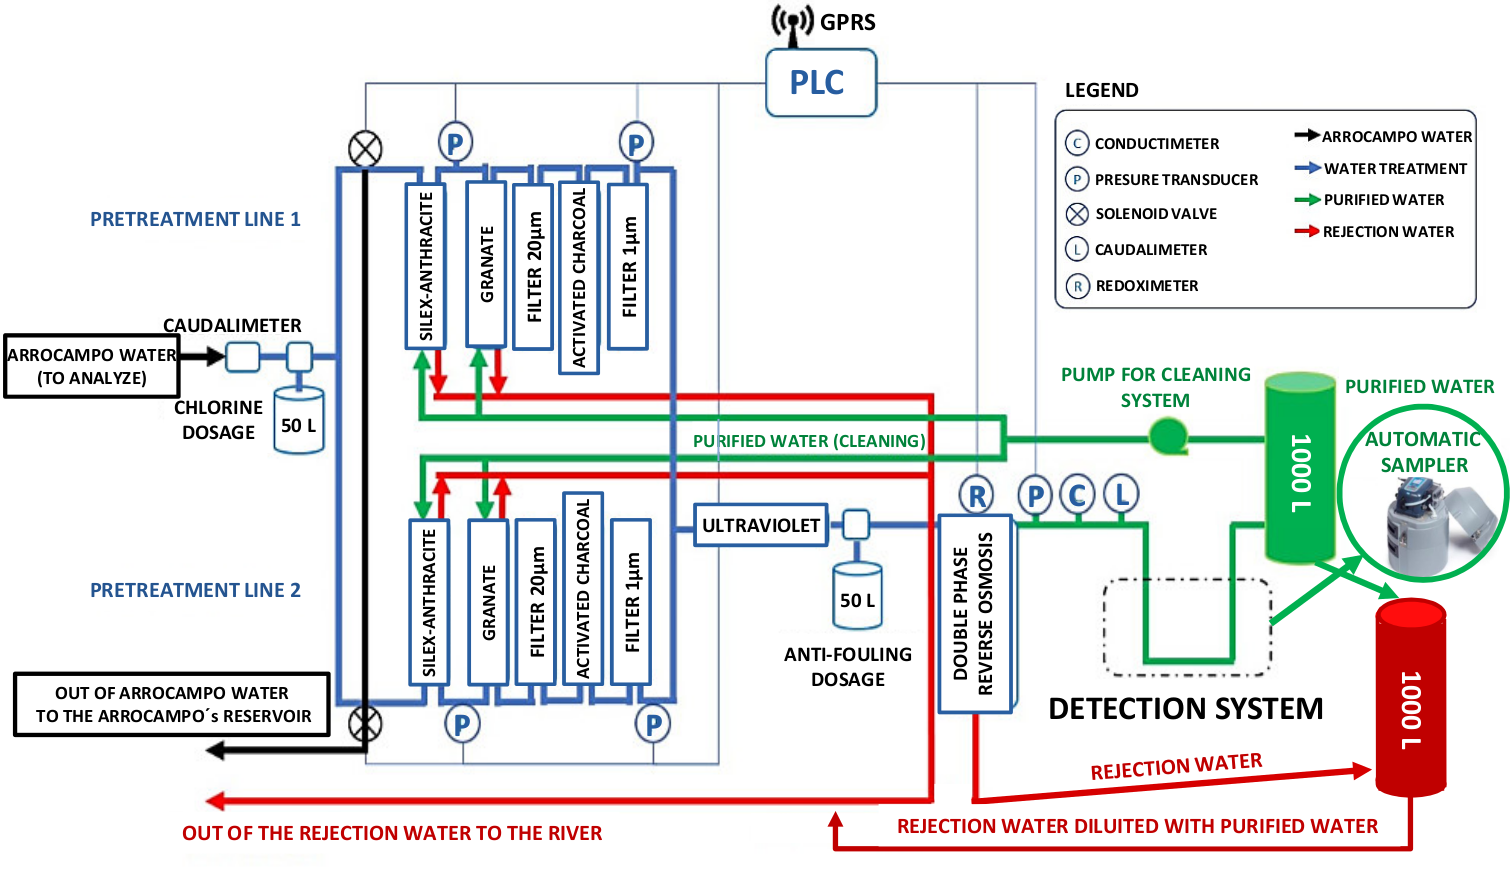
\includegraphics[scale=0.25]{3DesignPrinciples/33UltraPureWaterSystem/SchemeUltraPureWaterSystem.png}
\caption{Scheme of water purification system.\label{fig:WPSScheme}}
\end{figure}

This system has been installed in the Arrocampo dam and consists of four different consecutive stages:

\begin{enumerate}
\item{} First, the raw water from the Tagus River passes through two different filters, the first formed by Silex-Anthracite and the second by granate, with which a gross filtering is made (the largest particles are eliminated). This system has two parallel lines with this first stage which are capable of self-cleaning by injecting ultrapure water in the opposite direction.

\item{} Next, the outlet water sample of the first stage passes through a $20~\mu\meter$ filter (Formed by a synthetic mesh) and activated charcoal filters (one per line in both) that form the fine filtration stage. With the $20~\mu\meter$ filter the particles with diameters of up to $20\mu\meter$ are filtered and, with the activated charcoal filter, the chlorine and iron particles are removed.

\item{} Then, the outlet water sample of the second stage passes through the super-fine filtering consisting of a $1~\mu\meter$ filter, formed of a dense polypropylene mesh, (one per line), and UV lamps. The first filter removes all the particles up to diameters of $1~\mu\meter$ and, the UV lamps remove the organic matter present in the sample.

\item{} Finally, this water sample is introduced in the last stage, double-phase reverse osmosis, thereby reducing the conductivity of the water to values of $5~\mu$S$/\cm$. It was verified that a conductivity of $10~\mu$S$/\cm$ is achieved with only one module reverse osmosis, enough for the needed conditions of tritium detector. Therefore, just one module of reverse osmosis is used for $24~\hour$ and the other for another $24~\hour$, reducing the power consumption of the system.

\end{enumerate}

At the end of this system, each water sample is divided into two different outlet samples. The pure water sample, which is the ultrapure water that is introduced into tritium detector, and the rejection water, whose conductivity is even greater than the water sample before treatment because it contains all the particles that have been extracted from the ultrapure water sample.

The ultrapure water system is able to process up to $0.850~\meter^3/\hour$ with a single line operating or $1.480~\meter^3/\hour$ with both, greatly overestimating the requirements of the tritium detector. 

The software used for remote controlling the ultrapure water system is Siemens PLC, with which it can be controlled and the information about its status such as the state of the valves, the pressure probes or water production is obtained in real time. 

The appendix \ref{App:UltraPureWaterSystem} contains several photos about each part of this system, already installed in Arrocampo dam.